\documentclass[handout,hyperref={pdfpagelabels=false}]{beamer}
% \documentclass[hyperref={pdfpagelabels=false}]{beamer}

\usepackage[utf8x]{inputenc}
%\usepackage{default}

\usetheme{Antibes}
% \usetheme{Malmoe}

% \setbeamercovered{dynamic}

% trying to fix font warnings:
%\usepackage[utf8]{inputenc}
\usepackage[T1]{fontenc}
\usepackage{lmodern}
\usepackage{amsfonts}
\usepackage{amsmath}
\usepackage{amssymb}
\usepackage{type1cm} % fonts used by xfig generated figures needs that

\usepackage{multirow}

\usepackage{subfigure}

% Definition for subfloat to allow us to use listings/verbatim inside subfigures:
\newbox\subfigbox % Create a box to hold the subfigure. 
\makeatletter 
\newenvironment{subfloat}% % Create the new environment. 
{\def\caption##1{\gdef\subcapsave{\relax##1}}% 
\let\subcapsave=\@empty % Save the subcaption text. 
\let\sf@oldlabel=\label 
\def\label##1{\xdef\sublabsave{\noexpand\label{##1}}}% 
\let\sublabsave\relax % Save the label key. 
\setbox\subfigbox\hbox 
\bgroup}% % Open the box... 
{\egroup % ... close the box and call \subfigure. 
\let\label=\sf@oldlabel 
\subfigure[\subcapsave]{\box\subfigbox}}% 
\makeatother 



\usepackage{tikz}
\usepackage{tkz-graph}

\usetikzlibrary{arrows,%
                shapes,positioning}
\tikzstyle{node}=[circle,draw=blue!50!black!50,top color=white,bottom color=blue!50!black!25]
\tikzstyle{mynode}=[circle,draw=red!50!black!50,top color=white,bottom color=blue!50!black!25]
% \tikzstyle{user}=[ellipse,draw=green!50!black!50,top color=white,bottom color=green!50!black!25,densely dotted]


\author{Lloyd Brown}
\title{High-Performance Computing Networks at BYU}
\date{March 17, 2010}


\begin{document}

\frame{\titlepage}
\section{Outline}

  \frame{
    \tableofcontents
  }

\section{What is HPC?}

  \frame{
    \frametitle{What makes a supercomputer, super?}

    \begin{itemize}
      \pause\item Significantly larger compute capability than an average system
      \pause\item No specific threshold for capacity
      \pause\item Used to solve problems that are too large to easily be solved on a single, traditional system
      \pause\item May utilize specialty hardware and software
    \end{itemize}
  }

\section{Types of HPC}

  \frame{
    \frametitle{What kinds of HPC systems are out there?}
    There are two major categories of HPC systems:
    \begin{itemize}
      \pause\item Systems which utilize specialty hardware, including:
      \begin{itemize}
	\pause\item Processors
	\begin{itemize}
	  \pause\item Vector Processors (eg. Cray)
	  \pause\item Specialty Serial Processors (eg. Itanium, Power5, etc.)
	\end{itemize}
	\pause\item Accelerators
	\begin{itemize}
	  \pause\item GPUs
	  \pause\item FPGAs
	\end{itemize}
	\pause\item Specialty/Proprietary Interconnects
	\begin{itemize}
	  \pause\item Infiniband
	  \pause\item NUMALink
	  \pause\item Quadrics
	  \pause\item Myrinet
	\end{itemize}
% (eg. NUMALink, Infiniband, Quadrics, Myrinet, etc.)
      \end{itemize}
      \pause\item Commodity Hardware:
      \begin{itemize}
	\pause\item Stock processors (eg. x86, x86\_64)
	\pause\item Stock interconnects (Ethernet)
      \end{itemize}
    \end{itemize}

  }

\section{Infiniband}

  \frame{
    \frametitle{What is Infiniband?  And why do I care?}
    Infiniband is the most common high-performance interconnect used in HPC.  It:
    \begin{itemize}
      \pause\item is switched-fabric architecture (more like Fibre Channel than like Ethernet)
      \pause\item utilizes multiple speeds, lanes, and links
      \pause\item provides:
      \begin{itemize}
	\item extremely high bandwidth (commonly 40Gb/s)
	\pause\item extremely low latency (one-way < 10 $\mu$s, compared to approx. 32 $\mu$s for 1GbE)
      \end{itemize}
    \end{itemize}

  }

  \subsection{Terminology}

  \frame{
    \frametitle{Terms}
    \begin{itemize}
      \pause\item[HCA] Host Channel Adapter - The interface device that connects a host to the network
      \pause\item[GUID] Globally-unique Identifier; hardware address on each HCA or switch; like a MAC address
      \pause\item[LID] Logical Identifier (address) assigned by the subnet manager to the HCA; kinda like an IP, but resides in the upper part of layer 2
      \pause\item[SM] Subnet Manager, a hardware or software device that assigns LIDs to GUIDs, and pre-loads the switch forwarding tables
    \end{itemize}

  }

  \subsection{Physical Layer Characteristics}

  \frame{
    \frametitle{Lanes/Links/Speeds}
    Infiniband utilizes multiple lanes per physical link.  Each link has a certain speed based on the standard:

    \pause

    \begin{center}
     
      \begin{tabular}{|c|c|c|c|}
      \hline
		 & \emph{SDR} & \emph{DDR} & \emph{QDR}\\
      \hline
      \emph{1x}  & 2.5 Gb/s & 5 Gb/s & 10 Gb/s \\
      \hline
      \emph{4x}  & 10 Gb/s & 20 Gb/s & 40 Gb/s \\
      \hline
      \emph{12x} & 30 Gb/s & 60 Gb/s & 120 Gb/s \\
      \hline
      \end{tabular}
    \end{center}

  }

%   \frame{
%     \frametitle{Connectors}
%     
%   }

  \frame{
    \frametitle{Does this look familiar?}
    \begin{itemize}
      \item Is there any other common computer technology that looks like this from a physical layer?  Using multiple lanes, with per-lane speed doubling each successive iteration of the standard?\\
%     \pause Any gamers in the room?
%     \pause What is the most bandwidth and latency sensitive hardware used for gaming?  Requires the fastest communication?
%     \pause How about PCIe?
    
	

%       \pause\centering{How about}\centering{\pause\strong{PCIe}}
      \pause\item How about \emph{PCI-Express}?
    \end{itemize}
  }


  \subsection{Encoding}
    \frame{
      \frametitle{Encoding Overhead}
      The Infiniband standard uses an 8b/10b encoding, meaning that the net speed is 80\% of the raw speed:

      \pause

      \begin{center}
      
	\begin{tabular}{|c|c|c|c|}
	\hline
		                    & \emph{SDR}   & \emph{DDR}  & \emph{QDR}\\
	\hline
	\multirow{2}{*}{\emph{1x}}  & 2.5 Gb/s raw & 5 Gb/s raw  & 10 Gb/s raw \\
				    & 2 Gb/s net   & 4 Gb/s net  & 8 Gb/s net  \\
	\hline
	\multirow{2}{*}{\emph{4x}}  & 10 Gb/s raw  & 20 Gb/s raw & 40 Gb/s raw \\
				    & 8 Gb/s net   & 16 Gb/s net & 32 Gb/s net \\
	\hline
	\multirow{2}{*}{\emph{12x}} & 30 Gb/s raw  & 60 Gb/s raw & 120 Gb/s raw\\
				    & 24 Gb/s net  & 48 Gb/s net & 96 Gb/s net \\
	\hline
	\end{tabular}
      \end{center}
    }

  \subsection{Subnet Management}

    \frame{
      \frametitle{How Infiniband is Managed}
      Infiniband is designed as a trusted network.  The network is managed by a \emph{subnet manager} which does the following:
      \begin{itemize}
	\pause\item Periodically sweep the network, looking for topology changes, checking for errors, etc.
	\pause\item Build a cohesive model of the network topology
	\pause\item Load the switch forwarding tables with the LID/Port mapping
      \end{itemize}

    }

  \subsection{Topologies}
    \frame{
      \frametitle{Possible Topologies}
      \begin{itemize}
	\pause\item Tree/Fat-Tree
	\pause\item Fully-connected Mesh
	\pause\item Rectangular Mesh
	\pause\item Toroidal Mesh
% 	\pause\item Hypercube
	\pause\item Clos Network
      \end{itemize}
    }


    \frame{
      \frametitle{Fat Tree Example}
      \begin{center}
	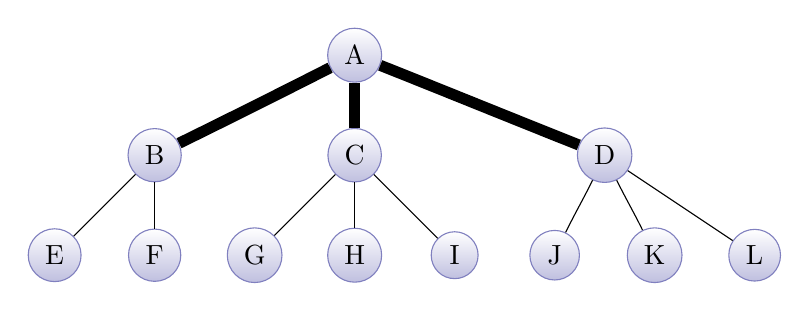
\begin{tikzpicture}[>=latex,line join=bevel,scale=0.5]
	%%
	\node (A) at (243bp,162bp) [node] {A};
	  \node (C) at (243bp,90bp) [node] {C};
	  \node (B) at (99bp,90bp) [node] {B};
	  \node (E) at (27bp,18bp) [node] {E};
	  \node (D) at (423bp,90bp) [node] {D};
	  \node (G) at (171bp,18bp) [node] {G};
	  \node (F) at (99bp,18bp) [node] {F};
	  \node (I) at (315bp,18bp) [node] {I};
	  \node (H) at (243bp,18bp) [node] {H};
	  \node (K) at (459bp,18bp) [node] {K};
	  \node (J) at (387bp,18bp) [node] {J};
	  \node (L) at (531bp,18bp) [node] {L};
	  \draw [] (C) ..controls (216bp,63bp) and (199bp,46bp)  .. (G);
	  \draw [] (D) ..controls (437bp,61bp) and (445bp,47bp)  .. (K);
	  \draw [] (C) ..controls (243bp,61bp) and (243bp,47bp)  .. (H);
	  \draw [] (D) ..controls (409bp,61bp) and (401bp,47bp)  .. (J);
	  \draw [] (C) ..controls (270bp,63bp) and (287bp,46bp)  .. (I);
	  \draw [] (D) ..controls (462bp,64bp) and (492bp,44bp)  .. (L);
	  \draw [line width=4bp] (A) ..controls (301bp,139bp) and (365bp,113bp)  .. (D);
	  \draw [] (B) ..controls (99bp,61bp) and (99bp,47bp)  .. (F);
	  \draw [line width=4bp] (A) ..controls (194bp,137bp) and (148bp,114bp)  .. (B);
	  \draw [] (B) ..controls (72bp,63bp) and (55bp,46bp)  .. (E);
	  \draw [line width=4bp] (A) ..controls (243bp,133bp) and (243bp,119bp)  .. (C);
	%

	%
	\end{tikzpicture}

      \end{center}
    }

  \frame{
    \frametitle{Fully-connected Mesh Example}
    \begin{center}
	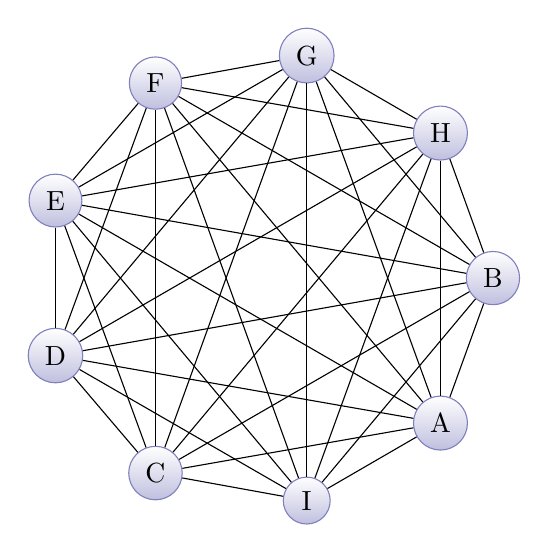
\begin{tikzpicture}[>=latex,line join=bevel,scale=0.45]
	  \node (A) at (336bp,81bp) [node] {A};
	  \node (C) at (108bp,41bp) [node] {C};
	  \node (B) at (378bp,197bp) [node] {B};
	  \node (E) at (28bp,259bp) [node] {E};
	  \node (D) at (28bp,135bp) [node] {D};
	  \node (G) at (229bp,375bp) [node] {G};
	  \node (F) at (108bp,353bp) [node] {F};
	  \node (I) at (229bp,19bp) [node] {I};
	  \node (H) at (336bp,313bp) [node] {H};
	  \draw [] (D) -- (H);
	  \draw [] (E) -- (F);
	  \draw [] (E) -- (I);
	  \draw [] (D) -- (G);
	  \draw [] (C) -- (I);
	  \draw [] (H) -- (I);
	  \draw [] (D) -- (E);
	  \draw [] (A) -- (F);
	  \draw [] (G) -- (I);
	  \draw [] (B) -- (F);
	  \draw [] (C) -- (D);
	  \draw [] (A) -- (B);
	  \draw [] (D) -- (I);
	  \draw [] (E) -- (H);
	  \draw [] (C) -- (H);
	  \draw [] (F) -- (G);
	  \draw [] (B) -- (G);
	  \draw [] (A) -- (E);
	  \draw [] (F) -- (H);
	  \draw [] (B) -- (C);
	  \draw [] (C) -- (G);
	  \draw [] (B) -- (H);
	  \draw [] (A) -- (D);
	  \draw [] (A) -- (I);
	  \draw [] (B) -- (D);
	  \draw [] (C) -- (F);
	  \draw [] (E) -- (G);
	  \draw [] (F) -- (I);
	  \draw [] (D) -- (F);
	  \draw [] (A) -- (C);
	  \draw [] (B) -- (I);
	  \draw [] (A) -- (G);
	  \draw [] (A) -- (H);
	  \draw [] (G) -- (H);
	  \draw [] (B) -- (E);
	  \draw [] (C) -- (E);
    %
    \end{tikzpicture}
  \end{center}
  }

  \frame{
    \frametitle{Rectangular/Toroidal Mesh Example}
    \begin{center}
      \begin{figure}
	\subfigure[Rectangular]{
	  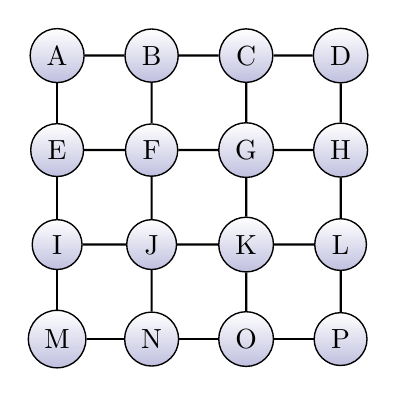
\begin{tikzpicture}[>=latex,line join=bevel,scale=1.2]
	    \GraphInit
      %       \SetVertexNormal[VertexStyle]
	    \Vertex[x=0,y=3,style=node]{A}
	    \Vertex[x=1,y=3,style=node]{B}
	    \Vertex[x=2,y=3,style=node]{C}
	    \Vertex[x=3,y=3,style=node]{D}
	    \Vertex[x=0,y=2,style=node]{E}
	    \Vertex[x=1,y=2,style=node]{F}
	    \Vertex[x=2,y=2,style=node]{G}
	    \Vertex[x=3,y=2,style=node]{H}
	    \Vertex[x=0,y=1,style=node]{I}
	    \Vertex[x=1,y=1,style=node]{J}
	    \Vertex[x=2,y=1,style=node]{K}
	    \Vertex[x=3,y=1,style=node]{L}
	    \Vertex[x=0,y=0,style=node]{M}
	    \Vertex[x=1,y=0,style=node]{N}
	    \Vertex[x=2,y=0,style=node]{O}
	    \Vertex[x=3,y=0,style=node]{P}
	    \Edge(A)(B)
	    \Edge(A)(E)
	    \Edge(B)(F)
	    \Edge(B)(C)
	    \Edge(C)(G)
	    \Edge(C)(D)
	    \Edge(D)(H)
	    \Edge(E)(F)
	    \Edge(E)(I)
	    \Edge(F)(G)
	    \Edge(F)(J)
	    \Edge(G)(H)
	    \Edge(G)(K)
	    \Edge(H)(L)
	    \Edge(I)(J)
	    \Edge(I)(M)
	    \Edge(J)(K)
	    \Edge(J)(N)
	    \Edge(K)(L)
	    \Edge(K)(O)
	    \Edge(L)(P)
	    \Edge(M)(N)
	    \Edge(N)(O)
	    \Edge(O)(P)
	  \end{tikzpicture}
	}%end of subfigure
	\subfigure[Toroidal]{
	  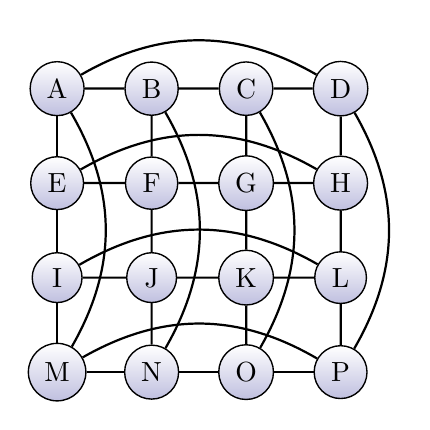
\begin{tikzpicture}[>=latex,line join=bevel,scale=1.2]
	    \GraphInit
      %       \SetVertexNormal[VertexStyle]
	    \Vertex[x=0,y=3,style=node]{A}
	    \Vertex[x=1,y=3,style=node]{B}
	    \Vertex[x=2,y=3,style=node]{C}
	    \Vertex[x=3,y=3,style=node]{D}
	    \Vertex[x=0,y=2,style=node]{E}
	    \Vertex[x=1,y=2,style=node]{F}
	    \Vertex[x=2,y=2,style=node]{G}
	    \Vertex[x=3,y=2,style=node]{H}
	    \Vertex[x=0,y=1,style=node]{I}
	    \Vertex[x=1,y=1,style=node]{J}
	    \Vertex[x=2,y=1,style=node]{K}
	    \Vertex[x=3,y=1,style=node]{L}
	    \Vertex[x=0,y=0,style=node]{M}
	    \Vertex[x=1,y=0,style=node]{N}
	    \Vertex[x=2,y=0,style=node]{O}
	    \Vertex[x=3,y=0,style=node]{P}
	    \Edge(A)(B)
	    \Edge(A)(E)
	    \Edge(B)(F)
	    \Edge(B)(C)
	    \Edge(C)(G)
	    \Edge(C)(D)
	    \Edge(D)(H)
	    \Edge(E)(F)
	    \Edge(E)(I)
	    \Edge(F)(G)
	    \Edge(F)(J)
	    \Edge(G)(H)
	    \Edge(G)(K)
	    \Edge(H)(L)
	    \Edge(I)(J)
	    \Edge(I)(M)
	    \Edge(J)(K)
	    \Edge(J)(N)
	    \Edge(K)(L)
	    \Edge(K)(O)
	    \Edge(L)(P)
	    \Edge(M)(N)
	    \Edge(N)(O)
	    \Edge(O)(P)

	    \Edge[style=bend right](D)(A)
	    \Edge[style=bend right](H)(E)
	    \Edge[style=bend right](L)(I)
	    \Edge[style=bend right](P)(M)
	    \Edge[style=bend right](M)(A)
	    \Edge[style=bend right](N)(B)
	    \Edge[style=bend right](O)(C)
	    \Edge[style=bend right](P)(D)
	  \end{tikzpicture}
	}%end of subfigure
      \end{figure}
    \end{center}
  }

  \frame{
    \frametitle{Clos Network Example}
    \begin{center}
      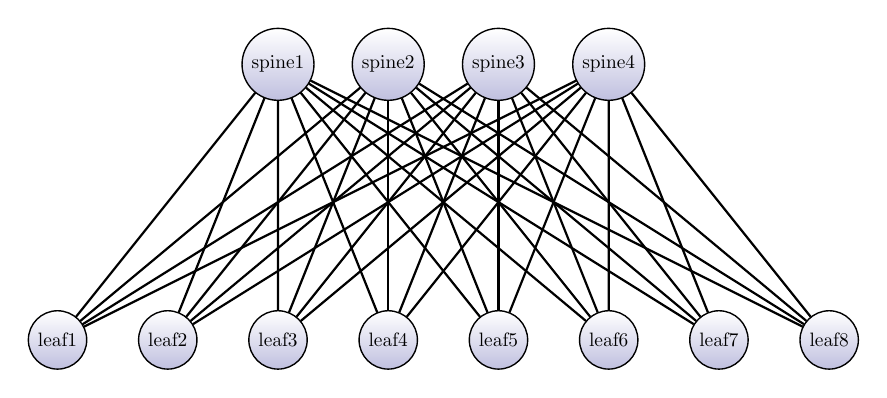
\begin{tikzpicture}[>=latex,line join=bevel,transform shape,scale=0.70]
	\GraphInit
	\Vertex[y=0,x=-3,style=node,L=spine1]{s1}
	\Vertex[y=0,x=-1,style=node,L=spine2]{s2}
	\Vertex[y=0,x=1,style=node,L=spine3]{s3}
	\Vertex[y=0,x=3,style=node,L=spine4]{s4}

	\Vertex[y=-5,x=-7,style=node,L=leaf1]{l1}
	\Vertex[y=-5,x=-5,style=node,L=leaf2]{l2}
	\Vertex[y=-5,x=-3,style=node,L=leaf3]{l3}
	\Vertex[y=-5,x=-1,style=node,L=leaf4]{l4}
	\Vertex[y=-5,x=1,style=node,L=leaf5]{l5}
	\Vertex[y=-5,x=3,style=node,L=leaf6]{l6}
	\Vertex[y=-5,x=5,style=node,L=leaf7]{l7}
	\Vertex[y=-5,x=7,style=node,L=leaf8]{l8}
	

	\Edge(s1)(l1)
	\Edge(s1)(l2)
	\Edge(s1)(l3)
	\Edge(s1)(l4)
	\Edge(s1)(l5)
	\Edge(s1)(l6)
	\Edge(s1)(l7)
	\Edge(s1)(l8)


	\Edge(s2)(l1)
	\Edge(s2)(l2)
	\Edge(s2)(l3)
	\Edge(s2)(l4)
	\Edge(s2)(l5)
	\Edge(s2)(l6)
	\Edge(s2)(l7)
	\Edge(s2)(l8)


	\Edge(s3)(l1)
	\Edge(s3)(l2)
	\Edge(s3)(l3)
	\Edge(s3)(l4)
	\Edge(s3)(l5)
	\Edge(s3)(l6)
	\Edge(s3)(l7)
	\Edge(s3)(l8)


	\Edge(s4)(l1)
	\Edge(s4)(l2)
	\Edge(s4)(l3)
	\Edge(s4)(l4)
	\Edge(s4)(l5)
	\Edge(s4)(l6)
	\Edge(s4)(l7)
	\Edge(s4)(l8)
      \end{tikzpicture}
    \end{center}

  }

  \frame{
    \frametitle{BYU Supercomputing's Clos Network}

    \begin{center}
      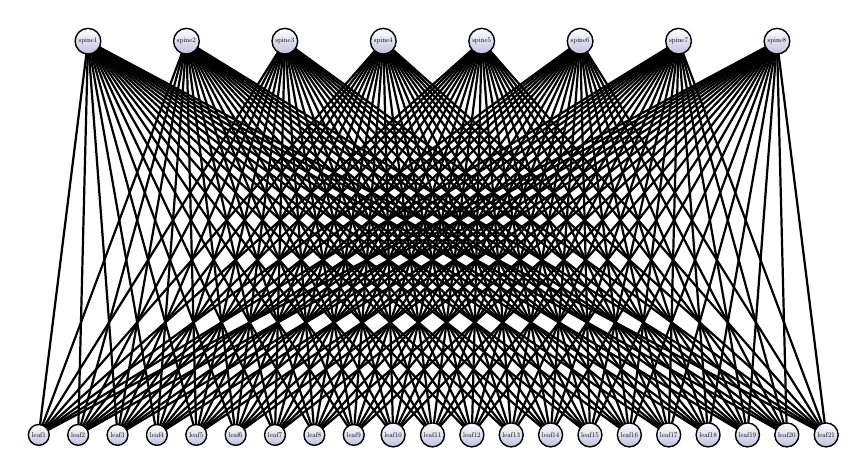
\begin{tikzpicture}[>=latex,line join=bevel,transform shape,scale=0.25]
	\GraphInit

	\Vertex[y=0,x=-17.5,style=node,L=spine1]{s1}
	\Vertex[y=0,x=-12.5,style=node,L=spine2]{s2}
	\Vertex[y=0,x=-7.5,style=node,L=spine3]{s3}
	\Vertex[y=0,x=-2.5,style=node,L=spine4]{s4}
	\Vertex[y=0,x=2.5,style=node,L=spine5]{s5}
	\Vertex[y=0,x=7.5,style=node,L=spine6]{s6}
	\Vertex[y=0,x=12.5,style=node,L=spine7]{s7}
	\Vertex[y=0,x=17.5,style=node,L=spine8]{s8}

	\Vertex[y=-20,x=-20,style=node,L=leaf1]{l1}
	\Vertex[y=-20,x=-18,style=node,L=leaf2]{l2}
	\Vertex[y=-20,x=-16,style=node,L=leaf3]{l3}
	\Vertex[y=-20,x=-14,style=node,L=leaf4]{l4}
	\Vertex[y=-20,x=-12,style=node,L=leaf5]{l5}
	\Vertex[y=-20,x=-10,style=node,L=leaf6]{l6}
	\Vertex[y=-20,x=-8,style=node,L=leaf7]{l7}
	\Vertex[y=-20,x=-6,style=node,L=leaf8]{l8}
	\Vertex[y=-20,x=-4,style=node,L=leaf9]{l9}
	\Vertex[y=-20,x=-2,style=node,L=leaf10]{l10}
	\Vertex[y=-20,x=0,style=node,L=leaf11]{l11}
	\Vertex[y=-20,x=2,style=node,L=leaf12]{l12}
	\Vertex[y=-20,x=4,style=node,L=leaf13]{l13}
	\Vertex[y=-20,x=6,style=node,L=leaf14]{l14}
	\Vertex[y=-20,x=8,style=node,L=leaf15]{l15}
	\Vertex[y=-20,x=10,style=node,L=leaf16]{l16}
	\Vertex[y=-20,x=12,style=node,L=leaf17]{l17}
	\Vertex[y=-20,x=14,style=node,L=leaf18]{l18}
	\Vertex[y=-20,x=16,style=node,L=leaf19]{l19}
	\Vertex[y=-20,x=18,style=node,L=leaf20]{l20}
	\Vertex[y=-20,x=20,style=node,L=leaf21]{l21}

	\Edge(s1)(l1)
	\Edge(s1)(l2)
	\Edge(s1)(l3)
	\Edge(s1)(l4)
	\Edge(s1)(l5)
	\Edge(s1)(l6)
	\Edge(s1)(l7)
	\Edge(s1)(l8)
	\Edge(s1)(l9)
	\Edge(s1)(l10)
	\Edge(s1)(l11)
	\Edge(s1)(l12)
	\Edge(s1)(l13)
	\Edge(s1)(l14)
	\Edge(s1)(l15)
	\Edge(s1)(l16)
	\Edge(s1)(l17)
	\Edge(s1)(l18)
	\Edge(s1)(l19)
	\Edge(s1)(l20)
	\Edge(s1)(l21)

	\Edge(s2)(l1)
	\Edge(s2)(l2)
	\Edge(s2)(l3)
	\Edge(s2)(l4)
	\Edge(s2)(l5)
	\Edge(s2)(l6)
	\Edge(s2)(l7)
	\Edge(s2)(l8)
	\Edge(s2)(l9)
	\Edge(s2)(l10)
	\Edge(s2)(l11)
	\Edge(s2)(l12)
	\Edge(s2)(l13)
	\Edge(s2)(l14)
	\Edge(s2)(l15)
	\Edge(s2)(l16)
	\Edge(s2)(l17)
	\Edge(s2)(l18)
	\Edge(s2)(l19)
	\Edge(s2)(l20)
	\Edge(s2)(l21)

	\Edge(s3)(l1)
	\Edge(s3)(l2)
	\Edge(s3)(l3)
	\Edge(s3)(l4)
	\Edge(s3)(l5)
	\Edge(s3)(l6)
	\Edge(s3)(l7)
	\Edge(s3)(l8)
	\Edge(s3)(l9)
	\Edge(s3)(l10)
	\Edge(s3)(l11)
	\Edge(s3)(l12)
	\Edge(s3)(l13)
	\Edge(s3)(l14)
	\Edge(s3)(l15)
	\Edge(s3)(l16)
	\Edge(s3)(l17)
	\Edge(s3)(l18)
	\Edge(s3)(l19)
	\Edge(s3)(l20)
	\Edge(s3)(l21)

	\Edge(s4)(l1)
	\Edge(s4)(l2)
	\Edge(s4)(l3)
	\Edge(s4)(l4)
	\Edge(s4)(l5)
	\Edge(s4)(l6)
	\Edge(s4)(l7)
	\Edge(s4)(l8)
	\Edge(s4)(l9)
	\Edge(s4)(l10)
	\Edge(s4)(l11)
	\Edge(s4)(l12)
	\Edge(s4)(l13)
	\Edge(s4)(l14)
	\Edge(s4)(l15)
	\Edge(s4)(l16)
	\Edge(s4)(l17)
	\Edge(s4)(l18)
	\Edge(s4)(l19)
	\Edge(s4)(l20)
	\Edge(s4)(l21)

	\Edge(s5)(l1)
	\Edge(s5)(l2)
	\Edge(s5)(l3)
	\Edge(s5)(l4)
	\Edge(s5)(l5)
	\Edge(s5)(l6)
	\Edge(s5)(l7)
	\Edge(s5)(l8)
	\Edge(s5)(l9)
	\Edge(s5)(l10)
	\Edge(s5)(l11)
	\Edge(s5)(l12)
	\Edge(s5)(l13)
	\Edge(s5)(l14)
	\Edge(s5)(l15)
	\Edge(s5)(l16)
	\Edge(s5)(l17)
	\Edge(s5)(l18)
	\Edge(s5)(l19)
	\Edge(s5)(l20)
	\Edge(s5)(l21)

	\Edge(s6)(l1)
	\Edge(s6)(l2)
	\Edge(s6)(l3)
	\Edge(s6)(l4)
	\Edge(s6)(l5)
	\Edge(s6)(l6)
	\Edge(s6)(l7)
	\Edge(s6)(l8)
	\Edge(s6)(l9)
	\Edge(s6)(l10)
	\Edge(s6)(l11)
	\Edge(s6)(l12)
	\Edge(s6)(l13)
	\Edge(s6)(l14)
	\Edge(s6)(l15)
	\Edge(s6)(l16)
	\Edge(s6)(l17)
	\Edge(s6)(l18)
	\Edge(s6)(l19)
	\Edge(s6)(l20)
	\Edge(s6)(l21)

	\Edge(s7)(l1)
	\Edge(s7)(l2)
	\Edge(s7)(l3)
	\Edge(s7)(l4)
	\Edge(s7)(l5)
	\Edge(s7)(l6)
	\Edge(s7)(l7)
	\Edge(s7)(l8)
	\Edge(s7)(l9)
	\Edge(s7)(l10)
	\Edge(s7)(l11)
	\Edge(s7)(l12)
	\Edge(s7)(l13)
	\Edge(s7)(l14)
	\Edge(s7)(l15)
	\Edge(s7)(l16)
	\Edge(s7)(l17)
	\Edge(s7)(l18)
	\Edge(s7)(l19)
	\Edge(s7)(l20)
	\Edge(s7)(l21)

	\Edge(s8)(l1)
	\Edge(s8)(l2)
	\Edge(s8)(l3)
	\Edge(s8)(l4)
	\Edge(s8)(l5)
	\Edge(s8)(l6)
	\Edge(s8)(l7)
	\Edge(s8)(l8)
	\Edge(s8)(l9)
	\Edge(s8)(l10)
	\Edge(s8)(l11)
	\Edge(s8)(l12)
	\Edge(s8)(l13)
	\Edge(s8)(l14)
	\Edge(s8)(l15)
	\Edge(s8)(l16)
	\Edge(s8)(l17)
	\Edge(s8)(l18)
	\Edge(s8)(l19)
	\Edge(s8)(l20)
	\Edge(s8)(l21)

      \end{tikzpicture}
    \end{center}

  }


%   \subsection{IB vs. Ethernet}
  
% 
\section{Building your own HPC Cluster}

  \frame{
    \frametitle{Components needed to build an HPC Cluster}

    To build your own HPC cluster, consider the following components:

    \begin{itemize}
%       \pause\item System Hardware
%       \pause\item Network Hardware
      \pause\item Hardware
      \pause\item Operating System Software
      \pause\item Infrastructure Software
      \pause\item Computational Software
    \end{itemize}

  }

  \subsection{Hardware}
    \frame{
      \frametitle{Hardware Considerations}
      When considering system hardware, be aware of the following considerations:
      \begin{itemize}
	\pause\item If a process is using resources on multiple nodes, it's significantly easier if the nodes' hardware is homogeneous.
	\pause\item You need to know the task's or software's requirements, and build the system appropriately in the following areas:
	\begin{itemize}
	  \pause\item Processor features and speed
	  \pause\item RAM
	  \pause\item Network Performance (bandwidth and latency)
	  \pause\item Storage requirements (total capacity, throughput, and IOPS)
	\end{itemize}
      \end{itemize}

    }
  \subsection{OS Software}

    \frame{
      \frametitle{Compute Node Operating System}
      \begin{itemize}
	\pause\item Each computational node needs to have a functioning operating system.  \emph{Linux} is the most common, usually installed either through a \emph{golden image} approach (usually vendor-provided), or scalable, scripted installer, eg. \emph{NPACI Rocks}.
	\pause\item You will need to make sure your computational software is supported on the system.  For example, many more commercial software packages run on \emph{RedHat Enterprise Linux} than on \emph{Ubuntu}.
      \end{itemize}

    }

  \subsection{Infrastructure Software}
    \frame{
      \frametitle{Organizing the effort}
      \begin{itemize}
	\pause\item If you're the only person using the system, you can just run your tasks directly.  If, however, you need to allow multiple users to have access, etc., you will probably need a queuing mechanism, eg. Moab/Torque, PBSPro, Slurm, SGE, LoadLeveler, LSF
	\pause\item You will need to monitor the system for hardware and software failures.  Think something like \emph{ganglia}.
      \end{itemize}
    }

  \subsection{Computational Software}
    \frame{
      \frametitle{Actually doing work}
      In order for the system to be useful, you need software to do some calculations.  Some things to consider here:
      \begin{itemize}
	\pause\item How will I get the software to utilize all the resources (eg. processors) available?  Do I need to use some form of communication framework like MPI to coordinate efforts, or will I just launch independent tasks
	\pause\item Is there any form of tuning that I can do to make the software more efficient?  For example, if it's compiled software, am I taking advantage of compilation optimizations, eg. SSE, or specialty BLAS implementations like Intel MKL or GotoBlas?
      \end{itemize}

    }


  \section{Summary/Conclusions}

  \frame{
    \frametitle{What does this all mean?}
    \begin{itemize}
      \pause\item In general, clusters of commodity hardware are the cheapest approaches to HPC, but it will vary depending on situation.
      \pause\item It is possible to set up a small HPC cluster without much hardware cost, or any real software cost.  Just don't expect anything \"{u}ber-cool like Infiniband.
      \pause\item You absolutely must understand your software, and its requirements
      \pause\item Not everything works like Ethernet and TCP/IP.  Network technologies like Fibre Channel and Infiniband throw away a number of the basic assumptions of Ethernet.
    \end{itemize}
  }

  \frame{
    \frametitle{Questions?}
%     Any questions?
  }


\end{document}
